\chapter{Historia madżonga}
% %%%%%%%%%%%%%%%%%%%%%%%%%%%%%%%%%%%%%%%%%%%%%%%%%%%%%%%%%%%%%%%%%%%%%%%%
% DEFINICJE
% %%%%%%%%%%%%%%%%%%%%%%%%%%%%%%%%%%%%%%%%%%%%%%%%%%%%%%%%%%%%%%%%%%%%%%%%
\section{Czym jest madżong?}
% %%%%%%%%%%%%%%%%%%%%%%%%%%%%%%%%%%%%%%%%%%%%
% DEFINICJA Z ENCYKLOPEDII
% %%%%%%%%%%%%%%%%%%%%%%%%%%%%%%%%%%%%%%%%%%%%%
\subsection{Powszechnie przyjęta definicja}
Madżong (麻将 \pinyin{májiàng} lub 麻雀 \pinyin{máquè}) to znana na całym świecie
gra dla czterech graczy pochodząca z Chin. Do gry używa się zestawu 144 kamieni
z wygrawerowanymi (niekiedy malowanymi) z jednej strony znakami chińskimi i
innymi symbolami. W trakcie rozgrywki gracze po kolei dobierają i odrzucają
kamienie w celu uzbierania jednego z ustalonych układów. Choć największą
popularność osiągnęła w Azji, ma również duże grupy odbiorców na pozostałych
kontynentach.
Istnieje kilkadziesiąt wariantów jej zasad, w większości powiązanych z
konkretnym regionem lub państwem. Rozbieżności pomiędzy zasadami poszczególnych
wariantów są w niektórych przypadkach bardzo duże, niektóre uwzględniają też grę
dla mniejszej liczby graczy (madżong dla trzech osób jest szczególnie popularny
w Japonii oraz Korei). (World Heritage Encyclopedia 2014)
% %%%%%%%%%%%%%%%%%%%%%%%%%%%%%%%%%%%%%%%%%%%%
% NAPOTKANE NIEŚCISŁOŚCI
% %%%%%%%%%%%%%%%%%%%%%%%%%%%%%%%%%%%%%%%%%%%%%
\subsection{Zastrzeżenia do definicji}
Autor pracy uważa, że powyższa definicja, choć poprawna, może nie być
wystarczająco precyzyjna na potrzeby niniejszej pracy.

Jedną z podstawowych nieścisłości jest określenie kamienia będącego częścią
zestawu do gry.
Niezależnie od tego, czy mówimy o kamieniach, płytkach domino czy też o kartach
używanych do bardzo różnego typu gier, określane są one w języku chińskim
wspólnym mianem \pinyin{pai} (牌 \pinyin{pái}). W wyniku tego, w wielu źródłach
autor nie może być pewien, czy opisywana gra wymagała kamieni, kart, czy jeszcze
innego typu elementów.

Innym problemem okazuje się być skład zestawu do gry. Wiele spośród
historycznych zestawów z terenu Chin różni się pomiędzy sobą typem i liczbą
figur w stopniu zdecydowanie większym, niż pozwalają na to uznane na terenie
Państwa Środka warianty zasad gry.

Kolejne wątpliwości wzbudza sposób gry. Niektóre ze źródeł sugerują, że
najstarsze zestawy do gry zbliżone w swoim składzie i wyglądzie do współczesnych
były wykorzystywane do gier innych niż madżong (czyli o zasadach
nieprzypominających żadnego ze współcześnie akceptowanych wariantów).

W związku z wymienionymi problemami autor decyduje się używać bardziej
precyzyjnej definicji gry (opisanej dalej w sekcji 1.1.3), która będzie
obowiązywać w niniejszej pracy.
% %%%%%%%%%%%%%%%%%%%%%%%%%%%%%%%%%%%%%%%%%%%%
% DEFINICJA OBOWIĄZUJĄCA W PRACY
% %%%%%%%%%%%%%%%%%%%%%%%%%%%%%%%%%%%%%%%%%%%%%
\subsection{Definicja przyjęta na potrzeby niniejszej pracy}
Madżong to gra spełniająca %definicję opisaną w sekcji 1.1.1 niniejszej pracy
%oraz 
następujące warunki:

%%%%%%%%%%%%%%%%%
% WARUNEK A
\begin{enumerate}[label={\alph*)}] \item Gra wykorzystuje zestaw składający się
z kamieni, które kształtem przypominają płytki domina, jednakże są nieco grubsze
i krótsze. Dopuszczalna jest także możliwość wykorzystywania kart zamiast
kamieni.
%%%%%%%%%%%%%%%%%
% WARUNEK B
\item Kamienie (lub karty) mają grawerowane lub malowane oznaczenia,
przyporządkowujące je do odpowiednich grup figur lub talii. Zestaw uwzględnia
następujące talie i figury\footnote{Talie i figury w sekcji 1.1.3 są opisane
skrótowo. Szczegółowy opis współczesnego zestawu do gry w madżonga znajduje się
w rozdziale 2.}:
	\begin{itemize}
	  \item 3 talie (kółka (筒 \pinyin{tǒng} lub 饼 \pinyin{bǐng}), bambusy (索
	  \pinyin{suǒ}) oraz znaki chińskie (万 \pinyin{wàn})) z kamieniami o
wartościach od 1 do 9; dopuszczalna jest także talia rang zamiast talii znaków
chińskich (oznaczana przez znaki 卐 (\pinyin{wàn}, dla kamienia o wartości 1)
oraz 品 (\pinyin{pǐn}, dla kamieni o wartościach od 2 do 9)); \item 4 wiatry
(wschód (東\footnote{\label{definicja_tradycyjne}Znaki wyjątkowo zapisane w formie
tradycyjnej, jako że w takiej występują na kamieniach. Dla znaku 東 forma
uproszczona to 东, dla 將 jest to 将, dla 發 -- 发, dla 龍 -- 龙, a dla 鳳 -- 凤.}
\pinyin{dōng}), południe (南 \pinyin{nán}), zachód (西 \pinyin{xī}) i północ (北 \pinyin{běi})); dopuszczalny jest także
wariant, w którym zamiast 4 wiatrów występuje 4 możnych (diuk (公 \pinyin{gōng}),
markiz (侯 \pinyin{hóu}), generał (將\footnotemark[2] \pinyin{jiàng}) oraz minister (相
\pinyin{xiàng}));
	  \item 3 smoki (biały (白 \pinyin{bái}), zielony (發\footnotemark[2]
	  \pinyin{fā}) i czerwony (中 \pinyin{zhòng})); dopuszczalny jest także wariant,
	  w którym zamiast smoka zielonego jest smok bez przydzielonej mu
	  barwy\footnote{,,3 Smoki'' w kolorach białym, zielonym i czerwonym to
	  zasadniczo termin zachodni, nie chiński.
	  Chińczycy używają określenia ,,3 \pinyin{yuan}'' (三元牌 \pinyin{sān yuán
	  pái}). We wczesnych zestawach do gry w madżonga występował jednakże
	  kamień oznaczany znakiem smoka -- 龍\footnotemark[2].} (龍\footnotemark[2]
	  \pinyin{lóng}), a zamiast smoka czerwonego -- feniks (鳳\footnotemark[2] \pinyin{fèng});
	  \item opcjonalnie kwiaty i/lub pory roku w różnej ilości;
	  \item opcjonalnie dżoker lub inne kamienie specjalne.
	\end{itemize}
%%%%%%%%%%%%%%%%%
% WARUNEK C
\item Kamienie o odpowiednich oznaczeniach występują w obrębie jednego zestawu
do gry w następujących ilościach:
	\begin{itemize}
	  \item 4 egzemplarze każdego z kamieni o numerach od 1 do 9 w każdej z 3 talii
	  (łącznie 108 kamieni);
	  \item 4 egzemplarze każdego z kamieni wiatrów (łącznie 16 kamieni)
	  \item 4 egzemplarze kamieni każdego z 3 smoków (łącznie 12 kamieni)
	  \item łączna liczba kamieni kwiatów i pór roku może się wahać od 0 do ponad
	  20;
	  \item łączna liczba kamieni specjalnych oraz dżokerów może się wahać od
	0 do ponad 20.
	\end{itemize} 
%%%%%%%%%%%%%%%%%
% WARUNEK D
\item Zasady gry uwzględniają następujące punkty:
	\begin{itemize}
	  \item gra polega na kompletowaniu przez graczy określonego przez zasady
	  układu kamieni zwanego dalej ,,ręką'';
	  \item gracz, który skompletuje gotową rękę jako pierwszy, wygrywa rozdanie;
	  \item choć liczba kamieni tworzących rękę może ulec zmianie w zależności od
	  wariantu gry, musi się ona składać z pewnej liczby ,,grup'' (pomniejszych
	  układów składających się z od 3 kamieni\footnote{Spotykane są również grupy
	  składające się z 4 lub 5 kamieni, jednakże wymagają one specjalnych
	  deklaracji w czasie gry oraz dobrania dodatkowych kamieni na wymianę. W
	  rezultacie, potencjalny czwarty lub piąty kamień w grupie nie wpływa na
	  budowę ręki, lecz na późniejsza punktację, stąd są one dalej traktowane
	  jako kamienie bonusowe.}) oraz dokładnie jednej pary (2 kamieni tego samego
	  typu), zgodnie z poniższym wzorem:
	  \begin{equation*}
	  n = 3g + 2 + x
	  \end{equation*}
	  gdzie n to liczba kamieni tworzących rękę, g to liczba grup, a x to liczba
	  kamieni bonusowych\footnote{Kamienie bonusowe nie zawsze są traktowane jako
	  część ręki gracza, jednakże są z nią ściśle powiązane, w związku z czym
	  autor pracy uznał za stosowne uwzględnić je we wzorze.} (kwiatów lub
	  rozszerzeń grup do 4 lub 5 kamieni);
	  \item gra jest skierowana do 4 graczy (opcjonalnie zasady mogą
	  zezwalać na grę dla 3 graczy).
	\end{itemize} 
\end{enumerate}
(Sloper 2006; Stanwick, Xu; Shìjiè Májiàng Zǔzhī 2006)
% %%%%%%%%%%%%%%%%%%%%%%%%%%%%%%%%%%%%%%%%%%%%%%%%%%%%%%%%%%%%%%%%%%%%%%%%
% POCZĄTKI
% %%%%%%%%%%%%%%%%%%%%%%%%%%%%%%%%%%%%%%%%%%%%%%%%%%%%%%%%%%%%%%%%%%%%%%%%
\section{Początki madżonga}
% %%%%%%%%%%%%%%%%%%%%%%%%%%%%%%%%%%%%%%%%%%%%
% L.L. HARR
% %%%%%%%%%%%%%%%%%%%%%%%%%%%%%%%%%%%%%%%%%%%%%
\subsection{Mity na temat starożytnych początków madżonga}
Nie jest kwestią prostą ustalenie od którego momentu w historii możemy mówić o
madżongu. Sprawa ta jest tym trudniejsza, że wiele powszechnie dostępnych źródeł
zawiera informacje nieprecyzyjne lub wręcz całkowicie błędne. 

Niezwykle popularnym, choć niewiele mającym wspólnego z rzeczywistością, jest
pogląd, że madżong jest grą niezwykle starą, pamiętającą czasy Konfucjusza,
czyli V wiek przed naszą erą. Ów pogląd wywodzi się z niesławnej publikacji Lew
Lysle Harra wydanej w 1922 roku pod tytułem ,,Pung Chow''\footnote{Tytuł książki
L.L. Harra ,,Pung Chow'' to jedna z popularniejszych nazw, jaką określano
madżonga w pierwszej połowie XX wieku. ,,Pung'' i ,,chow'' to przyjęty przez
Harra zapis 2 spośród najpopularniejszych ruchów dozwolonych w madżongu --
współcześnie są one znane jako \pinyin{peng} (碰 pèng) i \pinyin{chi} (吃 chī).}.
Lew Lysle Harr był w Chinach w 1919 roku reprezentantem amerykańskiej firmy
Graton and Knight Belting Company. Uznał on, że masowo produkowane zestawy do
madżonga w zunifikowanej, jednolitej formie pozwoliłoby na łatwą wymianę
zgubionych kamieni oraz byłyby łatwiejsze do sprzedaży.
Wyżej wymieniona publikacja to spisany przez niego podręcznik do nauki zasad
gry, który w swoim wstępie zawiera notatkę o historii i pochodzeniu madżonga.
Według jej treści, madżong w swojej pierwotnej postaci wymyślony został około
472 roku przed naszą erą na dworze króla państwa \pinyin{Wu}, czyli w okolicach
współczesnego \pinyin{Ningbo}\footnote{Ningbo (宁波 \pinyin{Níngbō}) - miasto we
wschodnich Chinach, w prowincji Zhejiang (浙江 \pinyin{Zhèjiāng}), port handlowy i
rybacki nad Morzem Wschodniochińskim.}. Madżong miał tam funkcjonować pod nazwą
\textit{Pe-Ling} jako gra umilająca czas samemu królowi, jego rodzinie i
bliskiemu otoczeniu. Karą za spędzanie w ten sposób czasu przez niższe warstwy
społeczeństwa była śmierć poprzez ścięcie głowy. Później dostęp do gry miał
zostać rozszerzony do kasty kupców, a dopiero w połowie XIX wieku naszej ery
stać się powszechnie dostępnym.
Publikacja prezentująca powyższe informacje miała służyć reklamie produktu,
który L.L. Harr zamierzał sprzedawać. Jako że zgodnie z ówczesnymi (jak
też i współczesnymi) badaniami nad pochodzeniem madżonga, gra nie istniała przed
XIX wiekiem naszej ery, a cała historia podana we wstępie do ,,Pung Chow'' była
nieprawdziwa, książka spotkała się z ostrą krytyką, a firma Harra zbankrutowała
w 1925 roku. Jednakże, choć L.L. Harr nie odniósł sukcesu w dziedzinie sprzedaży
madżonga, jego książka jest współcześnie powszechnie dostępna w księgarniach, a
ostra krytyka, z jaką się spotkała zaraz po jej pierwszej publikacji nie jest
wiedzą powszechną. W wyniku tego, że Harr faktycznie znajdował się w Chinach w
latach dwudziestych XX wieku, gdy madżong po raz pierwszy zaczął trafiać do
szerokiej publiczności w Europie i Ameryce Północnej, wiele źródeł uznaje jego
książkę za wiarygodną i odnosi się do zawartych w niej fałszywych informacji.
(Greenfield 2010; Harr 2008; Mah Jong Museum)
% %%%%%%%%%%%%%%%%%%%%%%%%%%%%%%%%%%%%%%%%%%%%
% FAKTYCZNE POCZĄTKI
% %%%%%%%%%%%%%%%%%%%%%%%%%%%%%%%%%%%%%%%%%%%%%
\subsection{Gry karciane - rzeczywiste początki madżonga}
Nawet po eliminacji źródeł zawierających informacje niewątpliwie fałszywe,
ustalenie dokładnego momentu pojawienia się madżonga po raz pierwszy pozostaje
kwestią trudną. Częścią problemu jest fakt, że madżong nie był wówczas grą
całkowicie nową, lecz kombinacją zasad szeregu funkcjonujących na terenie Chin w
XIX wieku i wcześniej hazardowych gier karcianych. Sprawa okazuje się być tym
bardziej skomplikowana w związku z tym, że gry hazardowe są w Chinach kwestią
wstydliwą, podobnie jak pisanie na ich temat. W czasie, gdy starsze gry karciane
powoli przekształcały się w grę nazywaną ,,madżongiem'', zainteresowanie tym
zagadnieniem ze strony chińskich uczonych było marginalne, a naukowcom z
pozostałych części świata nie było on znany aż do późnego XIX wieku.
Tym samym, wiele dat podawanych przez autora w dalszej części tego rozdziału
jest jedynie przybliżeniem.

% %%%%%%%%%%%%%%%% GRY KARCIANE
Jednakże, przed ustaleniem momentu pojawienia się madżonga należy poświęcić
uwagę również grom karcianym, z których prawdopodobnie się on wywodzi.

% %%%%%%%%%%%%%%%% SHIHU
Jedną z nich, która uznawana jest za spokrewnioną z madżongiem, jest
\pinyin{shihu} (十壶 \pinyin{shíhú}). Nazwę możnaby dosłownie przetłumaczyć jako
,,10 dzbanków'', choć spotykane jest także tłumaczenie ,,10 punktów'' (Stanwick,
Xu za Lo 2004). Można zatem przypuścić, że nazwę gry można również zapisać 十和
(\pinyin{shíhú}\footnote{Choć najczęstsze czytanie znaku 和 to ,,\pinyin{hé}'', a
znak ten najczęściej oznacza pokój, harmonię, a także występuje w zdaniu jako
spójnik, w kontekscie madżonga i wielu spokrewnionych z nim gier czytany jest on
,,\pinyin{hú}''. Oznacza on wówczas skompletowanie ręki, czyli zwycięstwo w
rozdaniu. Tym samym, prawdopodobnie najcelniejszym tłumaczeniem \pinyin{mohu}
jest ,,kompletowanie ręki w milczeniu''.}), czyli dosłownie ,,10 wygranych''. Do
gry służył zestaw kart papierowych, których liczba zazwyczaj wynosiła 120, choć
można było również spotkać warianty na 125, 132, a nawet 160 kart. Zestaw
składał się z:
\begin{itemize}
  \item 36 kart (4 egzemplarze każdego rodzaju karty) w każdej z 3 talii (餅
  \pinyin{bǐng}, 索 \pinyin{suǒ} oraz 万 \pinyin{wàn}), łącznie 108 kart;
  \item po 4 egzemplarze 3 kart kwiatów (花 \pinyin{huā}), łącznie 12 kart;
  \item rzadziej innych dodatkowych kart.
\end{itemize}
Jak łatwo zauważyć, choć skład takiego zestawu nie spełnia norm przyjętych w
madżongu, jest do nich bardzo zbliżony. Oznaczenia na kartach również odbiegają
od tych stosowanych w madżongu (Rysunek 1.1). Sama gra w \pinyin{shihu},
podobnie jak gra w madżonga, polegała na ułożeniu określonego układu w procesie
dobierania i odrzucania kart przez graczy po kolei. Zwycięski układ musiał być
wart minimum 10 punktów. \pinyin{Shihu} niewątpliwie zostało wymyślone przed
madżongiem, jako że jest wspominane w dziele pochodzącym z 1796 roku --
,,Malowane Łodzie Przyjemności z Yangzhou''\footnote{Tytułowe ,,łodzie
przyjemności'' to domy publiczne w Yangzhou (扬州 \pinyin{Yángzhōu}), mieście we
wschodnich Chinach. Klienci owych domów publicznych grywali w \pinyin{shihu},
nie jest jednakże jasnym, czy była to usługa świadczona przez same instytucje,
czy też zwyczajnie popularna w ich gronie rozrywka. (Stanwick, Xu)}
autorstwa \pinyin{Li Dou} (李斗, \pinyin{Lǐ Dǒu}).
(Stanwick, Xu)

\begin{figure}[h]
\centering
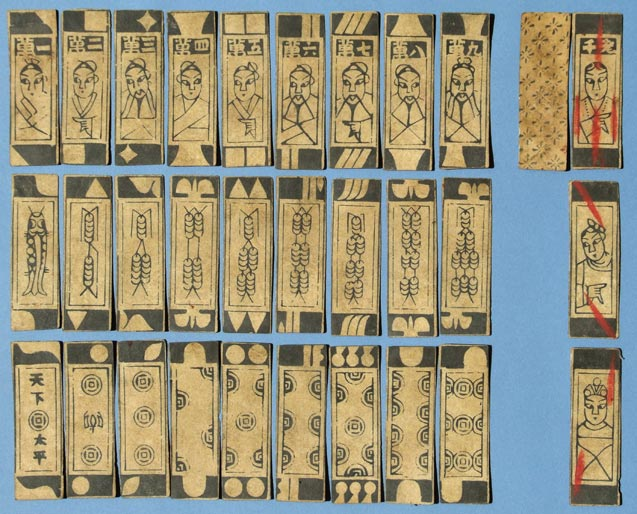
\includegraphics[width=0.75\textwidth]{1_shihu.jpg}
\caption{Niekompletny zestaw do gry w \pinyin{shihu}; 30 spośród 120 kart;
Chiny, ok. 1900 r;  źródło:
http://www.themahjongtileset.co.uk/tile-set-history/earliest-suit-names/}
\end{figure}

% MADIAO
Same karty używane do gry w \pinyin{shihu} wykorzystywane były również do wielu
innych gier, a ich wcześniejszym zastosowaniem prawdopodobnie była gra w
\pinyin{madiao} (馬吊 \pinyin{mǎdiào}), czyli dosłownie ,,wieszanie konia'',
pochodząca z czasu rządów cesarza Kangxi (康熙 Kāngxī), czyli z lat 1661--1722.
(Jin 1783) Zestaw \pinyin{madiao} składał się z 40 kart w 4 taliach -- czwarta
talia, niewystępująca w grach wywodzących się z \pinyin{madiao}, nazywana była
,,dziesiątkami myriad''. Później wykorzystywano zestawy zawierające tylko 3
talie (czyli 30 kart) do innych gier. (Stanwick, Xu)

%MOHU
Przykładem innej gry wykorzystującej zestaw do \pinyin{madiao} jest
\pinyin{mohu} (默和 \pinyin{mòhú}). Nazwę \pinyin{mohu} można dosłownie przetłumaczyć jako
,,układanie kart w ciszy''. Gra była przeznaczona dla 4 graczy i wymagała 60
kart (czyli najprawdopodobniej 2 zestawów kart \pinyin{madiao} pozbawionych
talii dziesiątków myriad). Jeden z graczy rozdawał wszystkim uczestnikom po
kolei po 1 karcie, aż każdy miał ich po 10. Następnie gracze układali je w
ciszy. Dalsza rozgrywka polegała na dobieraniu kart z pozostałych 20 w celu
ułożenia zwycięskiego układu (jeden z graczy, ale nie ten odpowiadający za
pierwsze rozdanie kart, rozdawał kolejne). (Jin 1783; Stanwick, Xu)
% 
% \footnote{,,Natrafianie na układ z
% kart'' to dosłowne znaczenie nazwy \pinyin{penghu}, jednakże prawdopodobnie jej
% pochodzenie jest nieco inne. \pinyin{Peng} (碰 \pinyin{pèng}) to jedna z
% najczęściej stosowanych deklaracji we współczesnym madżongu. Jej użycie pozwala
% na dobranie kamienia odrzuconego przez innego gracza do własnej trójki takich
% samych kamieni. Prawdopodobnie zachodzi związek pomiędzy tą nazwą, a nazwą gry w \pinyin{penghu}.}


% PENGHU
Inną tego typu grą jest \pinyin{penghu} (碰和 \pinyin{pènghú} -- dosłownie
,,natrafianie na układ z kart'').
W \pinyin{penghu} grano 4 lub 5 zestawami do \pinyin{madiao}, czyli łącznie 120
lub 150 kartami. (Stanwick, Xu) Inne źródło sugeruje, że stosowano 2 lub 2,5
zestawu do \pinyin{mohu} (Jin 1783), co sumuje się do tej samej liczby kart.
Nie jest oczywistym, czy gra wykształciła się bezpośrednio z \pinyin{madiao},
czy też pośrednio z \pinyin{mohu} (jak sugeruje Jin 1783).
Pojawiają się w niej układy występujące również we współczesnym madżongu, jak na
przykład \pinyin{peng}\footnote{\pinyin{peng} (碰 \pinyin{pèng}) to jedna z
 najczęściej stosowanych deklaracji we współczesnym madżongu. Jej użycie pozwala
 na dobranie kamienia odrzuconego przez innego gracza do własnej trójki takich
 samych kamieni. Występuje również w grze w \pinyin{penghu} i jest elementem jej
 nazwy.}. Można sądzić, że niektóre źródła mowiące tylko o \pinyin{shihu} lub
 tylko o \pinyin{penghu} nie rozróżniały tych dwóch gier, jako że ich zasady i
 skład zestawów do gry były do siebie zbliżone. (Jin 1783; Stanwick, Xu)

% PODSUMOWANIE KART
Karty do \pinyin{madiao} były również wykorzystywane do szeregu innych,
pomniejszych gier, jak \pinyin{kanhu} (看虎 \pinyin{kànhǔ} -- ,,obserwowanie
tygrysa''), \pinyin{hunjiang} (混江 \pinyin{hùnjiāng} -- ,,zwijanie rzeki'') oraz
\pinyin{suohu} (梭和 \pinyin{suōhú} - ,,układanie kart ruchem w tę i z
powrotem''). (Stanwick, Xu) Każda z nich jest warta wspomnienia, jako że wielu
pasjonatów oraz badaczy na przełomie XIX i XX wieku określało własne zestawy do
madżonga właśnie ich nazwami (nie będąc jeszcze świadomym różnicy).
Można wręcz przypuszczać, że funkcjonowały one przez długi czas równolegle z
nowo wykształconym madżongiem, a być może nawet grano w nie w przy pomocy
kamieni zamiast kart.
% %%%%%%%%%%%%%%%%%%%%%%%%%%%%%%%%%%%%%%%%%%%%
% MADŻONG NA PRZEŁOMIE XIX/XX WIEKU
% %%%%%%%%%%%%%%%%%%%%%%%%%%%%%%%%%%%%%%%%%%%%%
\subsection{Madżong pod koniec XIX wieku}
Ciężko określić, w którym dokładnie momencie zaczęto używać kamieni do gry
zamiast kart\footnote{Ze względu na nierozróżnianie ich w języku i określanie
wspólnym mianem \pinyin{pai}, zgodnie z zapisem w sekcji 1.1.2.}, jednakże było
to już niewątpliwie praktykowane w latach siedemdziesiątych XIX wieku. (Stanwick
2004) Niemiecki tłumacz Carl Himly w latach 1868-1876 zdobył zestaw bambusowych
kamieni, które w swoich publikacjach z 1889 i 1901 określał jako ,,bambusowe
\pinyin{pai} z Ningbo\footnote{Ningbo (宁波 \pinyin{Níngbō}) -- miasto we
wschodnich Chinach, w prowincji Zhejiang (浙江 Zhèjiāng), port handlowy i rybacki
nad Morzem Wschodniochińskim.}'' (宁波竹牌 \pinyin{Níngbō zhúpái}). Nie spełnia on
definicji madżonga przyjętej na potrzeby tej pracy (brakuje w nim kamieni
czerwonego oraz zielonego smoka), jednakże jest do niej bardzo zbliżony.
(Stanwick, Xu za Himly 1889-1901) Bardzo podobne zestawy (w których uwzględniony
już został smok czerwony, jednakże wciąż brakowało zielonego) pochodzące z
okresu pomiędzy 1869 a 1875 rokiem zostały dostarczone przez George'a B.
Glovera\footnote{George B. Glover, wicekonsul Stanów Zjednoczonych w Szanghaju w
latach 1858-1859. Później w latach od 1859 do około 1882 komisarz urzędu celnego
w różnych miejscach w Chinach.(Wikipedia 2013)} do Amerykańskiego Muzeum
Historii Naturalnej (American Museum of Natural History). (Stanwick 2004) Glover
napisał w 1875 roku notatkę, która została załączona do owych zestawów, w której
prawdopodobnie po raz pierwszy użyto poza Chinami nazwy
,,wróbel''\footnote{Glover w 1975 roku użył nazwy \pinyin{jiaqiao} (家雀
\pinyin{jiāqiǎo}), czyli dosłownie ,,wróbel domowy''. Współcześnie łatwiej można
spotkać określenie \pinyin{maque} (麻雀 \pinyin{máquè}), które również oznacza
wróbla, jednakże regionalnie można wciąż spotkać się także z użyciem tego słowa
jako synonim madżonga. W języku japońskim \pinyin{majian}, które zapisywane jest
tymi samymi znakami, co \pinyin{maque} po chińsku, również oznacza madżonga.
(Stanwick, Xu)}, która współcześnie jest jednym z wielu synonimów madżonga.
Zestawy różniły się pomiędzy sobą składem, jednakże można przyjąć że służyły do
tych samych lub spokrewnionych ze sobą gier. Jako że pochodziły z różnych
obszarów Chin -- Ningbo i Szanghaju, można przyjąć że stosowanie zestawów
kamieni zamiast kart stawało się w tym czasie coraz bardziej popularne w
Chinach.

Bardziej precyzyjne badania nad madżongiem rozpoczynają się w roku 1893,kiedy to
William Henry Wilkinson, pracownik konsulatu brytyjskiego w Chinach, wysłał
zbiór gier zakupionych w Chinach do profesora Stewarta Culina,\footnote{Stewart
Culin, amerykański etnograf, pracownik Uniwersytetu Pensylwanii, badacz gier,
ubioru i sztuki chińskiej; jeden z pierwszych badaczy madżonga. (Wikipedia
2016)} który Culin później wystawił na wystawie World's Colombian Exposition w
Chicago. W owym zbiorze znajdowała się gra karciana, którą Wilkinson określał
jako \pinyin{khanhoo}, czyli najprawdopodobniej wspomniane w sekcji 1.2.2
\pinyin{kanhu} (看虎 \pinyin{kànhǔ} -- ,,obserwowanie tygrysa'').
\pinyin{Khanhoo}, pośród innych gier wymienianych przez Wilkinsona, należało do
podzbioru określanego przez niego mianem ,,wróbli'', czyli \pinyin{maque}. Culin
zajął się badaniami na ten temat i w późniejszych publikacjach uznał ,,wróble''
Wilkinsona za przodków madżonga. (Culin 1924; Greenfield 2010)

% %%%%%%%%%%%%%%%%%%%%%%%%%%%%%%%%%%%%%%%%%%%%
% XX WIEK
% %%%%%%%%%%%%%%%%%%%%%%%%%%%%%%%%%%%%%%%%%%%%%
\section{Madżong w XX wieku}

% %%%%%%%%%%%%%%%%%%%%%%%
% SZANGHAJ 20s
% %%%%%%%%%%%%%%%%%%%%%%%
\subsection{Madżong w Szanghaju lat dwudziestych XX wieku}
Jakkolwiek \pinyin{khanhoo} cieszyło się zainteresowaniem naukowców, poza
terenem Chin nie zdobyło popularności. Przełomowy moment w historii madżonga nastąpił wtedy,
gdy gra trafiła do Szanghaju. Choć zasady sformułowane zostały w Ningbo, to
Szanghaj pozwolił im się w pełni rozwinąć i trafić do szerszego grona odbiorców.
W wyniku traktatów podpisanych po zakończeniu dziewiętnastowiecznych Wojen
opiumowych\footnote{Wojny opiumowe – wspólne określenie na mające miejsce w
dziewiętnastym wieku 2 konflikty zbrojne Chin z Wielką Brytanią i Francją;
jednym z ich skutków był szereg upokarzających dla Chin traktatów wymuszających
ustępstwa handlowe przy handlu wieloma towarami, przede wszystkim opium.}, port
w Szanghaju stanowił jedną ze specjalnie wyznaczonych stref, gdzie przybysze ze
Stanów Zjednoczonych, Wielkiej Brytanii i innych państw zachodnich mogły
dokonywać swobodnej wymiany kulturowej, niepodlegając chińskiemu prawu oraz
podatkom. (Greenfield 2010)

Sam Culin w 1909 roku w Szanghaju kupił „zestaw
domina wykonany z kości słoniowej”, który już spełniał definicję madżonga
przyjętą w sekcji 1.1.3. Możemy przyjąć, że wówczas podobne zestawy nie miały
jeszcze ustalonego składu, jako że według informatora nazwiskiem Dzau Sing
Chung z Szanghaju, na którego powołuje się Culin, były one
zazwyczaj wykonywane na zamówienie, zgodnie z potrzebami klienta. (Culin 1924)

Jednakże, dopóki zestaw do gry nie miał ustalonego składu i był wykonywany na
zamówienie, jego dystrybucja pozostawała problematyczna, w związku z czym szereg
osób dokonywało prób jego standaryzacji. Jedną z takich osób był Joseph A.
Babcock, reprezentant amerykańskiej firmy Standard Oil Company, który właśnie w
Szanghaju nauczył się grać w madżonga, by później
stać się najważniejszą osobą w historii popularyzacji tej gry na świecie. W
1920 roku wydał on pierwsze zasady gry w języku
angielskim, czyli ,,Czerwoną Księgę Zasad'' (\textit{Red Book of Rules}).
Książkę sprzedawano razem z zestawami do gry, którą początkowo importowano z
Chin, a później także wykonywano w Stanach Zjednoczonych. Babcock opatentował
nazwę ,,Mah-Jongg'', której różne pisownie (,,mahjong'', ,,majong'' i im
podobne) stały się powszechnie używaną na zachodzie nazwą gry. Określenie
,,madżong'', przyjęte na potrzeby niniejszej pracy, również jest jej
spolszczeniem. Wielu próbowało imitować sukces Babcocka, jednakże było
zmuszonych używać innych nazw gry, między innymi przez co nie odnieśli
porównywalnego sukcesu.\footnote{Dla przykładu, wspomniany w sekcji 1.2.1 Lew
Lysle Harr był zmuszony używać nazwy ,,Pung Chow''.} (Greenfield 2010)

\subsection{Odrodzenie madżonga}
Jako że madżong w swojej pierwotnej postaci był grą hazardową, kojarzącą się z
rozwiązłym stylem życia zepsutego zachodu, został on zakazany w 1966 roku na
początku rewolucji kulturalnej\footnote{Wielka proletariacka rewolucja
kulturalna – mający miejsce w latach 1966-1976 ruch społeczno-polityczny
zapoczątkowany przez przywódcę Partii Komunistycznej Chin, Mao Zedonga.}, wraz z
wszystkimi innymi przejawami hazardu na terenie całego kraju.
(Carlisle 2009)

Stworzono nowe zasady, które miały wyeliminować elementy gry hazardowej i
uzyskać grę, w której najważniejsze byłyby umiejętności gracza. Tym samym, w
1998 roku opublikowano ,,Międzynarodowy Standard Madżonga'' (国际标准麻将
\pinyin{guójì biāozhǔn májiàng}), czyli zasady międzynarodowe (w poszechnym użytku jest skrót
-- 国标麻将 \pinyin{guóbiāo májiàng}), a zakaz gry został zniesiony. W tym samym
roku madżong został w Chinach oficjalnie uznany za dyscyplinę sportową.
(Carlisle 2009, Zi 2015)

W 2002 roku w Tokio odbyły się pierwsze na świecie międzynarodowe zawody w grze
w madżonga, na których obowiązywały już zasady \pinyin{guóbiāo májiàng}.
Pierwotnie miały się one odbyć w Ningbo. Zwyciężył w nich reprezentant Japonii,
Mai Hatsune. (Kanazawa 2010, Nihon kenkō asa shō kyōkai kōshiki saito 2002)

W październiku 2005 roku w Pekinie utworzono Światową Organizację Madżonga
(World Mahjong Organization lub 世界麻将组织 \pinyin{Shìjiè Májiàng Zǔzhī}).
Poza Chinami, do krajów założycielskich należały między innymi Japonia, Stany
Zjednoczone Ameryki Północnej, Niemcy, Francja, Dania, Holandia oraz Węgry.
(Shìjiè Májiàng Zǔzhī 2006)

W listopadzie 2007 roku w Chengdu\footnote{成都 (\pinyin{Chéngdū}) -- stolica
prowincji 四川 (\pinyin{Sìchuān}), miasto w południowo-wschodnich Chinach.} odbyły
się pierwsze oficjalne Światowe Mistrzostwa Madżonga. Od tego czasu stało się to
regularnym wydarzeniem - kolejne miały miejsce w 2010 roku w
Utrecht\footnote{Utrecht --  miasto w środkowej Holandii.} oraz w 2012 w
Chongqing\footnote{重庆 (\pinyin{Chóngqìng}) -- miasto w środkowych Chinach, jedno
z czterech miast wydzielonych Chińskiej Republiki Ludowej.}. (Kǒuzhuāng Bāshì
2014)






 














